\label{ch:implementation}

Besides the realization of EDA sensors results relatively simple when compared with the circuitry of other devices, its limited diffusion at present implies a series of issues that are required to be addressed. More specifically:

\begin{itemize}
    \item EDA wearables oriented to research purposes tend to be particularly expensive (and most of the time unaffordable for small research projects)
    \item Well-known devices implementing EDA-related features do not provide Application Programming Interfaces for developers and do not provide open-source solutions either
\end{itemize}

The following chapter describes the implementation of a \textbf{simple} and completely \textbf{open-source} wearable device, aimed at providing a low-cost framework for the Electrodermal Activity measurement in experimental contexts.

\section{BITalino Electrodermal Activity Sensor}\label{sec:bitalino}

The sensor unit employed is the purpose-built \textbf{Electrodermal Activity Sensor} by \textbf{BITalino}. This constitutes a single module provided by the company aimed at composing, along with many others, the \textbf{BITalino (r)evolution Board Kit} \cite{bitalino-general}, an all-in-one device implementing a custom firmware for the collection and aggregation of data retrieved from multiple biosensors. Besides all the features implemented by these boards result interesting in research contexts, the main drawbacks are related to the lack of mobility that the device would cause, which is a primary concern within the bounds of fall detection systems.

On that basis, a single EDA module was purchased for a 25,00 € (Tax Excluded) price and a minimal Arduino-based firmware was implemented in order to retrieve measurements from the individual unit without having to rely on third-party solutions.

\subsection{Description and Features}\label{sec:bitalino-features}

The EDA sensor module consists of a breakout boards whose dimensions correspond to 12mm x 27mm \cite{bitalino-general}. A complete list of informations regarding the configuration of the unit is reported in Table \ref{toc:bitalino-features} .

\begin{table}[H]
\centering
\begin{tabular}{ll}
    \hline
    Parameter               & Value \\
    \hline
    Current                 & DC \\
    Range                   & 0-30 $\mu S$ \\
    Consumption             & $\pm 0.1 mA$ \\
    Bandwidth               & 0 - 2.8 Hz \\
    Measurement             & continuous \\
    Input Voltage Range     & 1.8 - 5.5 V \\
    \hline
\end{tabular}
\caption{Characteristics of the BITalino EDA sensor unit}
\label{toc:bitalino-features}
\end{table}

Furthermore, the device is sold in the three following configurations, according to the requirements of the customers: 

\begin{itemize}
    \item Self-assemble
    \item Self-assemble with UC-E6 connectors
    \item Assembled
\end{itemize}

The first version consists of the single breakout board and requires manual soldering of both the electrodes and connectors, while the second one provides pre-installed UC-E6 connectors in order to facilitate the connection of the electrodes and the main board. The assembled version provides, instead, a ready-made configuration consisting on: 

\begin{itemize}
    \item Pre-soldered electrodes
    \item Pre-soldered UC-E6 cable
    \item A 3D printed ABS case containing the breakout board
\end{itemize}

% https://bitalino.com/storage/uploads/media/homeguide4-eda.pdf

In order to exploit the convenience of both the ABS case and the pre-soldered electrodes cables, a pre-assembled unit was acquired and later modified in order to implement the connection with a third-party microcontroller. More specifically, the modification procedure consisted in the following steps: 

\begin{enumerate}
    \item Open the ABS case
    \item Unsolder the four UC-E6 connector cables from their respective pins on the breakout board
    \item Solder a dupont cable on each one of the pins
    \item Widen the cable conduit of the ABS case in order to allow the passage of the previously soldered dupont cables
    \item Close the ABS case again
\end{enumerate}


% \begin{figure}[h]
%     \centering
%     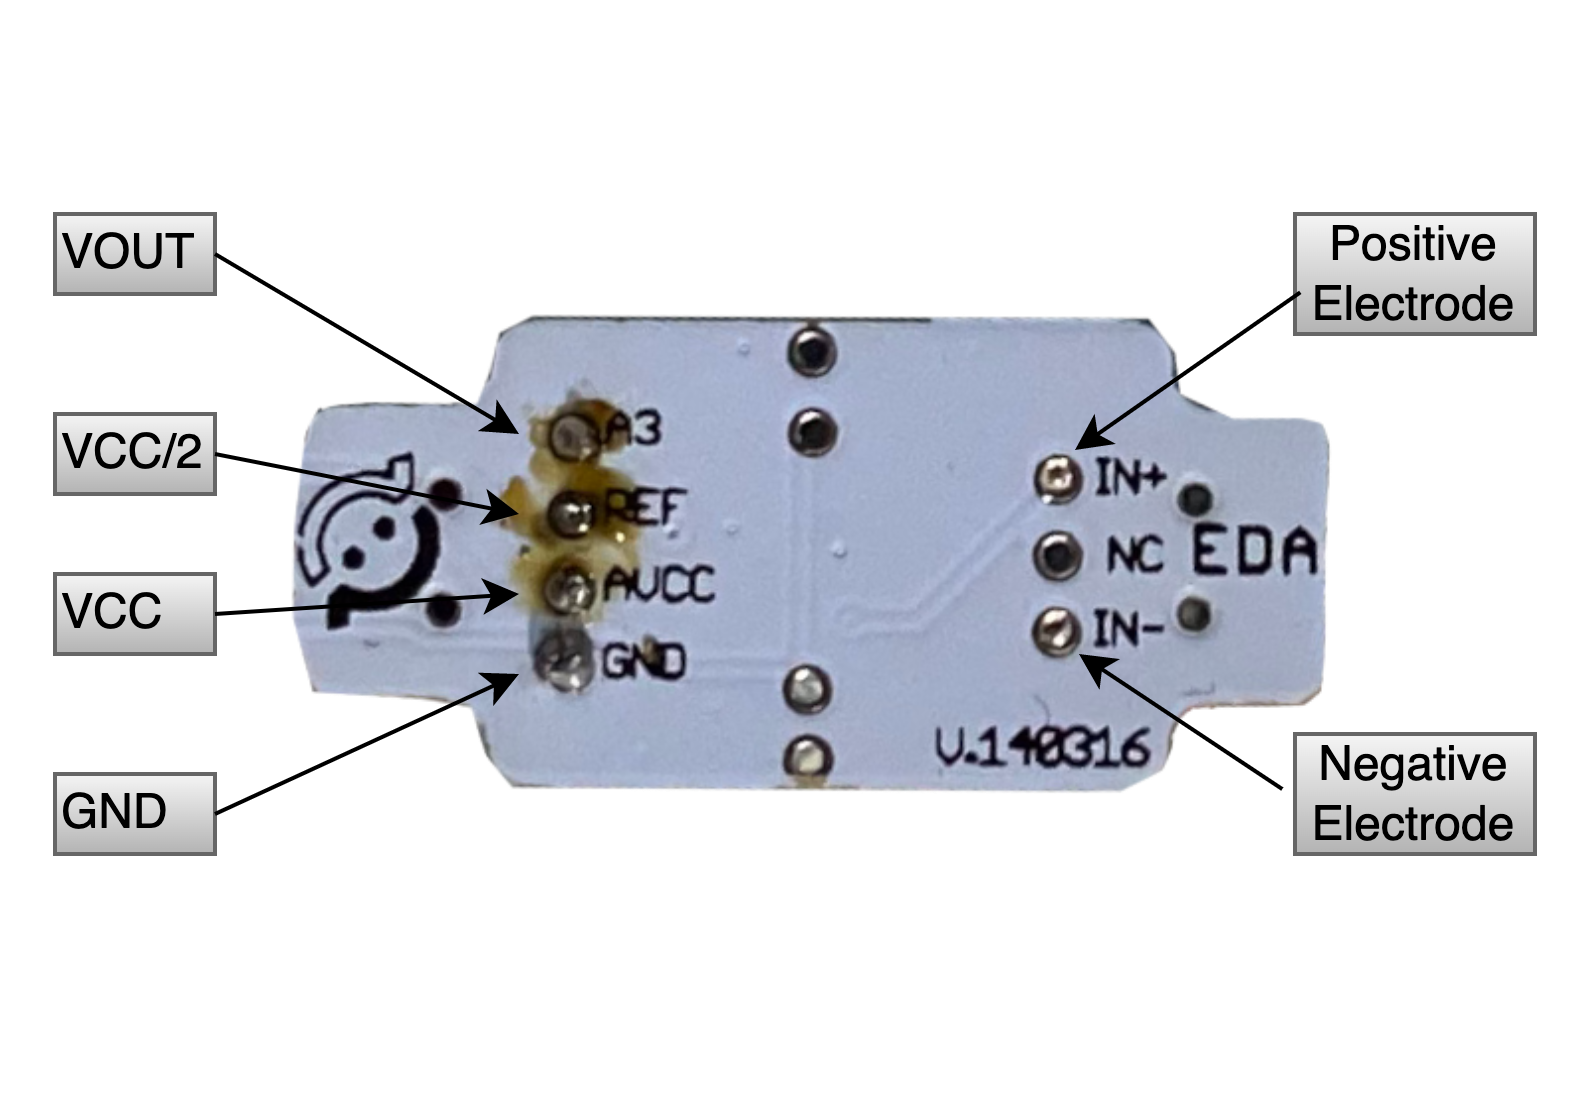
\includegraphics[width=3cm]{./images/bitalino.drawio.png}
%     \caption{Decomposition of Raw EDA signal in its two components}
%     \label{fig:eda-example}
% \end{figure}





